\documentclass[tikz]{standalone}

\usetikzlibrary{arrows.meta,positioning}

\begin{document}
	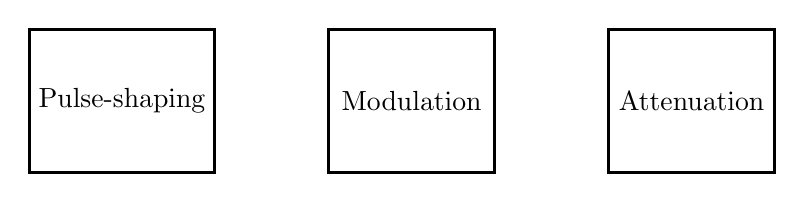
\begin{tikzpicture}[
		node distance=4em,
		arrow/.style={-latex},
		block/.style={draw, very thick, fill=white, minimum height=12ex, minimum width=6em, align=center},
	]
		\coordinate (in) at (0,0);
		\node (psh) [block, right=of in] {Pulse-shaping};
		\node (mod) [block, right=of psh] {Modulation};
		\node (att) [block, right=of mod] {Attenuation};
		\coordinate[right=of att] (out);
	\end{tikzpicture}
\end{document}
